
            \begin{tabular}{ll}
    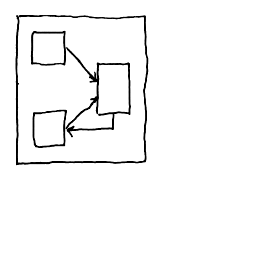
\includegraphics[width = 5cm]{../TikZ/drawings/expert-0.png}&
    
        \begin{minipage}{10cm}
        \begin{verbatim}
  line(6,2,6,3,arrow = False,solid = True)
  line(6,2,3,2,arrow = True,solid = True)
  rectangle(0,0,8,9)
  rectangle(5,3,7,6)
        reflect(y = 9)
        line(3,7,5,5,arrow = True,solid = True)
        rectangle(1,6,3,8)
        \end{verbatim}
\end{minipage}

    \end{tabular}        
            \\

            \begin{tabular}{ll}
    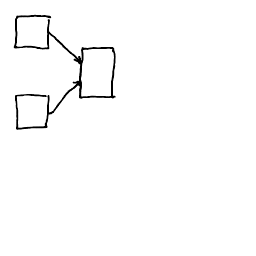
\includegraphics[width = 5cm]{../TikZ/drawings/expert-2.png}&
    
        \begin{minipage}{10cm}
        \begin{verbatim}
  rectangle(4,2,6,5)
        reflect(y = 7)
        line(2,6,4,4,arrow = True,solid = True)
        rectangle(0,5,2,7)
        \end{verbatim}
\end{minipage}

    \end{tabular}        
            \\

            \begin{tabular}{ll}
    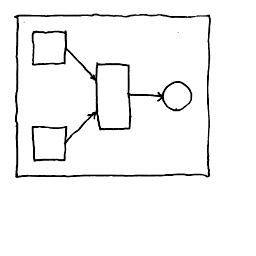
\includegraphics[width = 5cm]{../TikZ/drawings/expert-3.png}&
    
        \begin{minipage}{10cm}
        \begin{verbatim}
  circle(10,5)
  line(3,2,5,4,arrow = True,solid = True)
    for (2)
        line(-4*i + 7,3*i + 5,-4*i + 9,5,arrow = True,solid = True)
        rectangle(-5*i + 5,-3*i + 3,5*i + 7,3*i + 7)
        rectangle(1,6*i + 1,3,6*i + 3)
        \end{verbatim}
\end{minipage}

    \end{tabular}        
            \\

            \begin{tabular}{ll}
    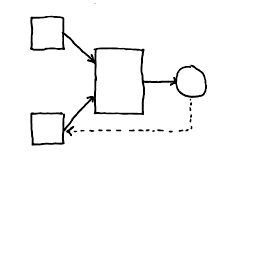
\includegraphics[width = 5cm]{../TikZ/drawings/expert-4.png}&
    
        \begin{minipage}{10cm}
        \begin{verbatim}
  circle(10,4)
  line(10,1,10,3,arrow = False,solid = False)
  line(10,1,2,1,arrow = True,solid = False)
  rectangle(4,2,7,6)
        reflect(y = 8)
        line(2,1,4,3,arrow = True,solid = True)
        line(7,4,9,4,arrow = True,solid = True)
        rectangle(0,0,2,2)
        \end{verbatim}
\end{minipage}

    \end{tabular}        
            \\

            \begin{tabular}{ll}
    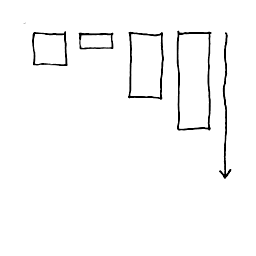
\includegraphics[width = 5cm]{../TikZ/drawings/expert-5.png}&
    
        \begin{minipage}{10cm}
        \begin{verbatim}
  line(12,9,12,0,arrow = True,solid = True)
    for (2)
        rectangle(3*i + 6,-2*i + 5,3*i + 8,9)
        rectangle(3*i,7,3*i + 2,9)
        \end{verbatim}
\end{minipage}

    \end{tabular}        
            \\

            \begin{tabular}{ll}
    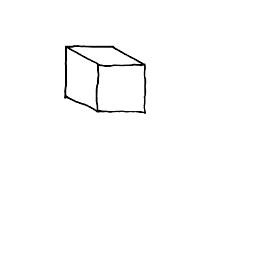
\includegraphics[width = 5cm]{../TikZ/drawings/expert-6.png}&
    
        \begin{minipage}{10cm}
        \begin{verbatim}
  line(0,4,3,4,arrow = False,solid = True)
  rectangle(2,0,5,3)
    for (2)
        line(3*i,3*i + 1,3*i + 2,3*i,arrow = False,solid = True)
        line(0,-3*i + 4,-2*i + 2,3,arrow = False,solid = True)
        \end{verbatim}
\end{minipage}

    \end{tabular}        
            \\

            \begin{tabular}{ll}
    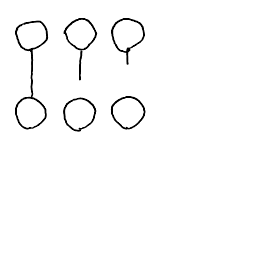
\includegraphics[width = 5cm]{../TikZ/drawings/expert-7.png}&
    
        \begin{minipage}{10cm}
        \begin{verbatim}
  for (3)
      circle(3*i + 1,6)
      circle(-3*i + 7,1)
      line(-3*i + 7,-1*i + 4,-3*i + 7,5,arrow = False,solid = True)
        \end{verbatim}
\end{minipage}

    \end{tabular}        
            \\

            \begin{tabular}{ll}
    
\includegraphics[width = 5cm]{../TikZ/drawings/expert-8.png}&
    
        \begin{minipage}{10cm}
        \begin{verbatim}
  line(0,0,0,4,arrow = False,solid = True)
        \end{verbatim}
\end{minipage}

    \end{tabular}        
            \\

            \begin{tabular}{ll}
    
\includegraphics[width = 5cm]{../TikZ/drawings/expert-9.png}&
    
        \begin{minipage}{10cm}
        \begin{verbatim}
  line(6,0,0,0,arrow = True,solid = True)
        \end{verbatim}
\end{minipage}

    \end{tabular}        
            \\

            \begin{tabular}{ll}
    
\includegraphics[width = 5cm]{../TikZ/drawings/expert-10.png}&
    
        \begin{minipage}{10cm}
        \begin{verbatim}
  rectangle(0,0,3,4)
        \end{verbatim}
\end{minipage}

    \end{tabular}        
            \\

            \begin{tabular}{ll}
    
\includegraphics[width = 5cm]{../TikZ/drawings/expert-11.png}&
    
        \begin{minipage}{10cm}
        \begin{verbatim}
  circle(1,1)
        \end{verbatim}
\end{minipage}

    \end{tabular}        
            \\

            \begin{tabular}{ll}
    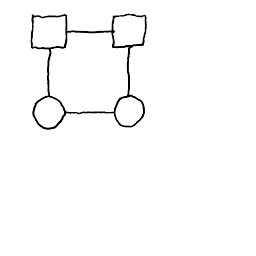
\includegraphics[width = 5cm]{../TikZ/drawings/expert-12.png}&
    
        \begin{minipage}{10cm}
        \begin{verbatim}
  for (2)
      circle(-5*i + 6,1)
      line(2,5*i + 1,5,5*i + 1,arrow = False,solid = True)
      line(5*i + 1,2,5*i + 1,5,arrow = False,solid = True)
      rectangle(-5*i + 5,5,-5*i + 7,7)
        \end{verbatim}
\end{minipage}

    \end{tabular}        
            \\

            \begin{tabular}{ll}
    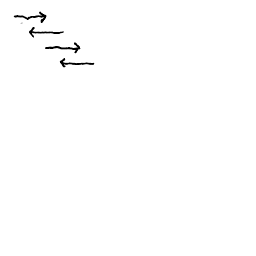
\includegraphics[width = 5cm]{../TikZ/drawings/expert-13.png}&
    
        \begin{minipage}{10cm}
        \begin{verbatim}
  line(2,1,4,1,arrow = True,solid = True)
  line(5,0,3,0,arrow = True,solid = True)
  line(0,3,2,3,arrow = True,solid = True)
  line(3,2,1,2,arrow = True,solid = True)
        \end{verbatim}
\end{minipage}

    \end{tabular}        
            \\

            \begin{tabular}{ll}
    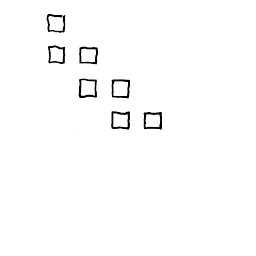
\includegraphics[width = 5cm]{../TikZ/drawings/expert-14.png}&
    
        \begin{minipage}{10cm}
        \begin{verbatim}
  rectangle(6,0,7,1)
    for (3)
        rectangle(-2*i + 4,2*i + 2,-2*i + 5,2*i + 3)
        rectangle(-2*i + 4,2*i,-2*i + 5,2*i + 1)
        \end{verbatim}
\end{minipage}

    \end{tabular}        
            \\

            \begin{tabular}{ll}
    
\includegraphics[width = 5cm]{../TikZ/drawings/expert-15.png}&
    
        \begin{minipage}{10cm}
        \begin{verbatim}
  line(3,0,5,0,arrow = False,solid = True)
  line(2,1,4,1,arrow = False,solid = False)
  line(0,3,2,3,arrow = False,solid = False)
  line(1,2,3,2,arrow = False,solid = True)
        \end{verbatim}
\end{minipage}

    \end{tabular}        
            \\

            \begin{tabular}{ll}
    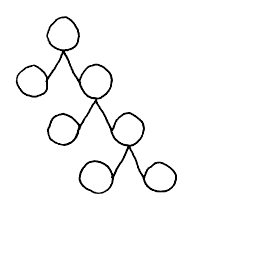
\includegraphics[width = 5cm]{../TikZ/drawings/expert-16.png}&
    
        \begin{minipage}{10cm}
        \begin{verbatim}
  circle(9,1)
    for (3)
        circle(2*i + 3,-3*i + 10)
        circle(2*i + 1,-3*i + 7)
        line(-2*i + 6,3*i + 1,-2*i + 7,3*i + 3,arrow = False,solid = True)
        line(-2*i + 7,3*i + 3,-2*i + 8,3*i + 1,arrow = False,solid = True)
        \end{verbatim}
\end{minipage}

    \end{tabular}        
            \\

            \begin{tabular}{ll}
    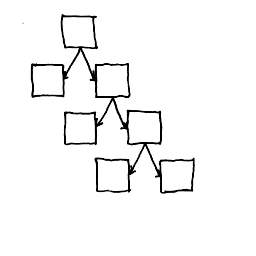
\includegraphics[width = 5cm]{../TikZ/drawings/expert-17.png}&
    
        \begin{minipage}{10cm}
        \begin{verbatim}
  rectangle(8,0,10,2)
    for (3)
        line(-2*i + 7,3*i + 3,-2*i + 8,3*i + 1,arrow = True,solid = True)
        line(2*i + 3,-3*i + 9,2*i + 2,-3*i + 7,arrow = True,solid = True)
        rectangle(-2*i + 6,3*i + 3,-2*i + 8,3*i + 5)
        rectangle(-2*i + 4,3*i,-2*i + 6,3*i + 2)
        \end{verbatim}
\end{minipage}

    \end{tabular}        
            \\

            \begin{tabular}{ll}
    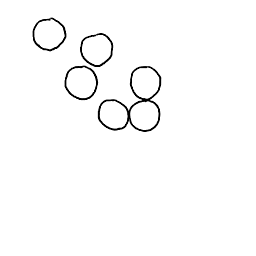
\includegraphics[width = 5cm]{../TikZ/drawings/expert-18.png}&
    
        \begin{minipage}{10cm}
        \begin{verbatim}
  for (2)
      circle(-1*i + 4,-2*i + 5)
      circle(-6*i + 7,3*i + 3)
      circle(-2*i + 7,1)
        \end{verbatim}
\end{minipage}

    \end{tabular}        
            \\

            \begin{tabular}{ll}
    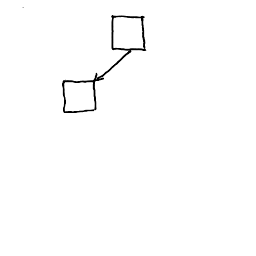
\includegraphics[width = 5cm]{../TikZ/drawings/expert-19.png}&
    
        \begin{minipage}{10cm}
        \begin{verbatim}
  line(4,4,2,2,arrow = True,solid = True)
  rectangle(3,4,5,6)
  rectangle(0,0,2,2)
        \end{verbatim}
\end{minipage}

    \end{tabular}        
            \\

            \begin{tabular}{ll}
    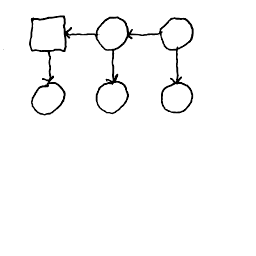
\includegraphics[width = 5cm]{../TikZ/drawings/expert-20.png}&
    
        \begin{minipage}{10cm}
        \begin{verbatim}
  rectangle(0,4,2,6)
    for (2)
        circle(4*i + 5,4*i + 1)
        line(4*i + 4,5,4*i + 2,5,arrow = True,solid = True)
              reflect(x = 10)
              circle(4*i + 5,-4*i + 5)
              line(4*i + 5,4,4*i + 5,2,arrow = True,solid = True)
        \end{verbatim}
\end{minipage}

    \end{tabular}        
            \\

            \begin{tabular}{ll}
    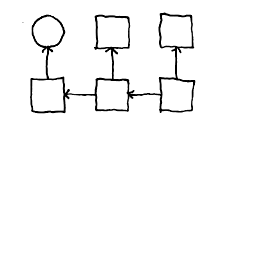
\includegraphics[width = 5cm]{../TikZ/drawings/expert-21.png}&
    
        \begin{minipage}{10cm}
        \begin{verbatim}
  circle(1,5)
    for (2)
        line(-4*i + 8,1,-4*i + 6,1,arrow = True,solid = True)
        rectangle(4*i + 4,4*i,4*i + 6,4*i + 2)
              reflect(x = 10)
              line(-4*i + 5,2,-4*i + 5,4,arrow = True,solid = True)
              rectangle(4*i,4*i,4*i + 2,4*i + 2)
        \end{verbatim}
\end{minipage}

    \end{tabular}        
            \\

            \begin{tabular}{ll}
    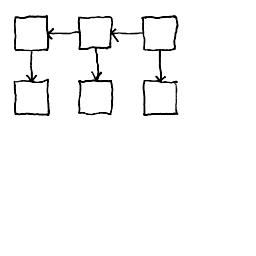
\includegraphics[width = 5cm]{../TikZ/drawings/expert-22.png}&
    
        \begin{minipage}{10cm}
        \begin{verbatim}
  line(4,5,2,5,arrow = True,solid = True)
  line(8,5,6,5,arrow = True,solid = True)
    for (3)
        line(4*i + 1,4,4*i + 1,2,arrow = True,solid = True)
        rectangle(4*i,0,4*i + 2,2)
        rectangle(-4*i + 8,4,-4*i + 10,6)
        \end{verbatim}
\end{minipage}

    \end{tabular}        
            \\

            \begin{tabular}{ll}
    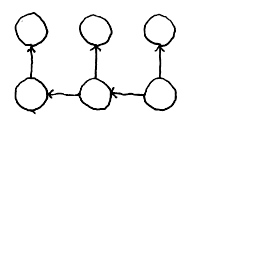
\includegraphics[width = 5cm]{../TikZ/drawings/expert-23.png}&
    
        \begin{minipage}{10cm}
        \begin{verbatim}
  for (2)
      line(-4*i + 8,1,-4*i + 6,1,arrow = True,solid = True)
            reflect(x = 10)
            circle(5,-4*i + 5)
            circle(-8*i + 9,4*i + 1)
            line(-4*i + 9,2,-4*i + 9,4,arrow = True,solid = True)
        \end{verbatim}
\end{minipage}

    \end{tabular}        
            \\

            \begin{tabular}{ll}
    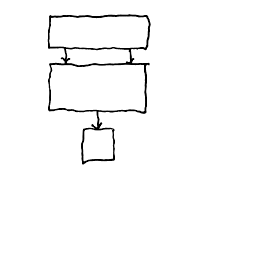
\includegraphics[width = 5cm]{../TikZ/drawings/expert-24.png}&
    
        \begin{minipage}{10cm}
        \begin{verbatim}
  line(5,7,5,6,arrow = True,solid = True)
  rectangle(2,0,4,2)
    for (2)
        line(2*i + 1,-4*i + 7,2*i + 1,-4*i + 6,arrow = True,solid = True)
        rectangle(0,4*i + 3,6,3*i + 6)
        \end{verbatim}
\end{minipage}

    \end{tabular}        
            \\

            \begin{tabular}{ll}
    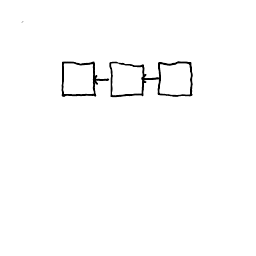
\includegraphics[width = 5cm]{../TikZ/drawings/expert-25.png}&
    
        \begin{minipage}{10cm}
        \begin{verbatim}
  line(3,1,2,1,arrow = True,solid = True)
  rectangle(6,0,8,2)
        reflect(x = 5)
        line(6,1,5,1,arrow = True,solid = True)
        rectangle(3,0,5,2)
        \end{verbatim}
\end{minipage}

    \end{tabular}        
            \\

            \begin{tabular}{ll}
    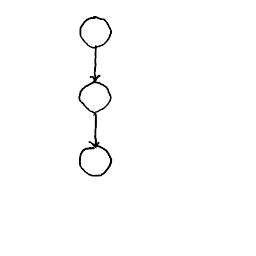
\includegraphics[width = 5cm]{../TikZ/drawings/expert-26.png}&
    
        \begin{minipage}{10cm}
        \begin{verbatim}
  line(1,3,1,4,arrow = False,solid = True)
  line(1,3,1,2,arrow = True,solid = True)
  line(1,8,1,6,arrow = True,solid = True)
    for (3)
        circle(1,4*i + 1)
        \end{verbatim}
\end{minipage}

    \end{tabular}        
            \\

            \begin{tabular}{ll}
    
\includegraphics[width = 5cm]{../TikZ/drawings/expert-27.png}&
    
        \begin{minipage}{10cm}
        \begin{verbatim}
      line(0,1,1,0,arrow = False,solid = True)
      line(1,2,2,1,arrow = False,solid = True)
        \end{verbatim}
\end{minipage}

    \end{tabular}        
            \\

            \begin{tabular}{ll}
    
\includegraphics[width = 5cm]{../TikZ/drawings/expert-28.png}&
    
        \begin{minipage}{10cm}
        \begin{verbatim}
  line(0,2,2,2,arrow = False,solid = True)
  line(0,0,0,2,arrow = False,solid = True)
        \end{verbatim}
\end{minipage}

    \end{tabular}        
            \\

            \begin{tabular}{ll}
    
\includegraphics[width = 5cm]{../TikZ/drawings/expert-29.png}&
    
        \begin{minipage}{10cm}
        \begin{verbatim}
  for (3)
      line(0,-1*i + 6,2*i + 2,-1*i + 6,arrow = False,solid = True)
      line(-1*i + 2,2*i,-1*i + 2,4,arrow = False,solid = True)
        \end{verbatim}
\end{minipage}

    \end{tabular}        
            \\

            \begin{tabular}{ll}
    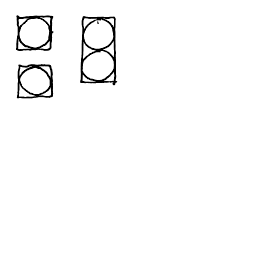
\includegraphics[width = 5cm]{../TikZ/drawings/expert-30.png}&
    
        \begin{minipage}{10cm}
        \begin{verbatim}
  rectangle(0,0,2,2)
    for (2)
        circle(1,-3*i + 4)
        circle(5,-2*i + 4)
        rectangle(-4*i + 4,2*i + 1,-4*i + 6,5)
        \end{verbatim}
\end{minipage}

    \end{tabular}        
            \\

            \begin{tabular}{ll}
    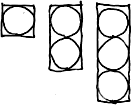
\includegraphics[width = 5cm]{../TikZ/drawings/expert-31.png}&
    
        \begin{minipage}{10cm}
        \begin{verbatim}
  circle(4,3)
    for (3)
        circle(-3*i + 7,5)
        circle(7,-2*i + 5)
        rectangle(-3*i + 6,2*i,-3*i + 8,6)
        \end{verbatim}
\end{minipage}

    \end{tabular}        
            \\

            \begin{tabular}{ll}
    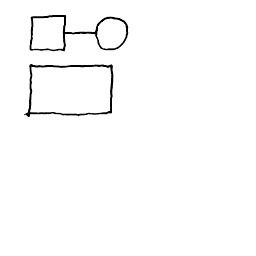
\includegraphics[width = 5cm]{../TikZ/drawings/expert-32.png}&
    
        \begin{minipage}{10cm}
        \begin{verbatim}
  circle(5,5)
  line(2,5,4,5,arrow = False,solid = True)
  rectangle(0,4,2,6)
  rectangle(0,0,5,3)
        \end{verbatim}
\end{minipage}

    \end{tabular}        
            \\

            \begin{tabular}{ll}
    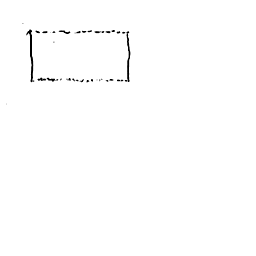
\includegraphics[width = 5cm]{../TikZ/drawings/expert-33.png}&
    
        \begin{minipage}{10cm}
        \begin{verbatim}
  line(0,3,6,3,arrow = False,solid = False)
  line(0,0,0,3,arrow = False,solid = True)
  line(0,0,6,0,arrow = False,solid = False)
  line(6,0,6,3,arrow = False,solid = True)
        \end{verbatim}
\end{minipage}

    \end{tabular}        
            \\

            \begin{tabular}{ll}
    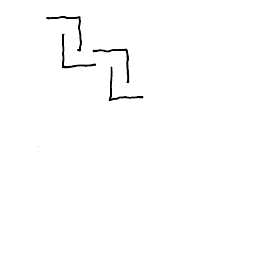
\includegraphics[width = 5cm]{../TikZ/drawings/expert-34.png}&
    
        \begin{minipage}{10cm}
        \begin{verbatim}
  for (2)
      line(-1*i + 2,-1*i + 3,-1*i + 2,-1*i + 5,arrow = False,solid = True)
      line(3,-3*i + 3,5,-3*i + 3,arrow = False,solid = True)
      line(4*i,-5*i + 5,2*i + 2,-3*i + 5,arrow = False,solid = True)
      line(-4*i + 5,1,-2*i + 5,-1*i + 3,arrow = False,solid = True)
        \end{verbatim}
\end{minipage}

    \end{tabular}        
            \\

            \begin{tabular}{ll}
    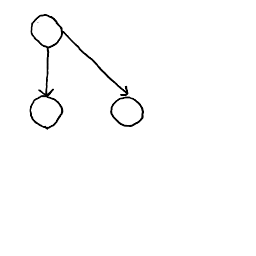
\includegraphics[width = 5cm]{../TikZ/drawings/expert-35.png}&
    
        \begin{minipage}{10cm}
        \begin{verbatim}
  circle(1,6)
    for (2)
        circle(-5*i + 6,1)
        line(-1*i + 2,-1*i + 6,-5*i + 6,2,arrow = True,solid = True)
        \end{verbatim}
\end{minipage}

    \end{tabular}        
            \\

            \begin{tabular}{ll}
    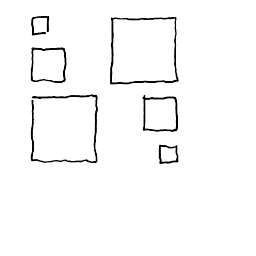
\includegraphics[width = 5cm]{../TikZ/drawings/expert-36.png}&
    
        \begin{minipage}{10cm}
        \begin{verbatim}
  for (2)
      rectangle(-8*i + 8,5*i,-7*i + 9,6*i + 1)
      rectangle(0,-8*i + 8,3*i + 1,-5*i + 9)
      rectangle(-2*i + 7,3*i + 2,9,5*i + 4)
        \end{verbatim}
\end{minipage}

    \end{tabular}        
            \\

            \begin{tabular}{ll}
    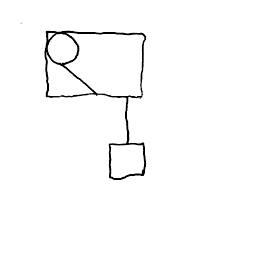
\includegraphics[width = 5cm]{../TikZ/drawings/expert-37.png}&
    
        \begin{minipage}{10cm}
        \begin{verbatim}
  circle(1,8)
    for (2)
        line(-4*i + 5,5*i + 2,-2*i + 5,5,arrow = False,solid = True)
        rectangle(4*i,-5*i + 5,6,-7*i + 9)
        \end{verbatim}
\end{minipage}

    \end{tabular}        
            \\

            \begin{tabular}{ll}
    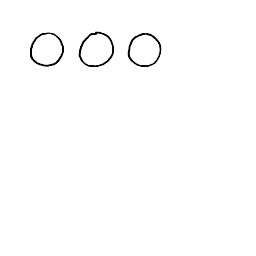
\includegraphics[width = 5cm]{../TikZ/drawings/expert-40.png}&
    
        \begin{minipage}{10cm}
        \begin{verbatim}
  circle(4,1)
        reflect(x = 8)
        circle(1,1)
        \end{verbatim}
\end{minipage}

    \end{tabular}        
            \\

            \begin{tabular}{ll}
    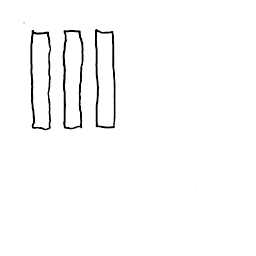
\includegraphics[width = 5cm]{../TikZ/drawings/expert-41.png}&
    
        \begin{minipage}{10cm}
        \begin{verbatim}
  rectangle(0,0,1,6)
  rectangle(4,0,5,6)
  rectangle(2,0,3,6)
        \end{verbatim}
\end{minipage}

    \end{tabular}        
            \\

            \begin{tabular}{ll}
    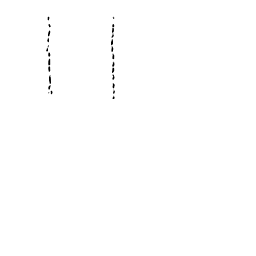
\includegraphics[width = 5cm]{../TikZ/drawings/expert-42.png}&
    
        \begin{minipage}{10cm}
        \begin{verbatim}
  line(4,1,4,5,arrow = False,solid = False)
  line(4,0,4,1,arrow = False,solid = False)
  line(0,0,0,5,arrow = False,solid = False)
        \end{verbatim}
\end{minipage}

    \end{tabular}        
            \\

            \begin{tabular}{ll}
    
\includegraphics[width = 5cm]{../TikZ/drawings/expert-43.png}&
    
        \begin{minipage}{10cm}
        \begin{verbatim}
  line(0,0,0,5,arrow = False,solid = True)
  line(4,0,4,5,arrow = False,solid = True)
        \end{verbatim}
\end{minipage}

    \end{tabular}        
            \\

            \begin{tabular}{ll}
    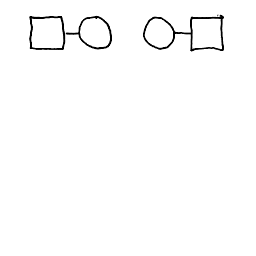
\includegraphics[width = 5cm]{../TikZ/drawings/expert-44.png}&
    
        \begin{minipage}{10cm}
        \begin{verbatim}
      reflect(x = 12)
      circle(4,1)
      line(9,1,10,1,arrow = False,solid = True)
      rectangle(0,0,2,2)
        \end{verbatim}
\end{minipage}

    \end{tabular}        
            \\

            \begin{tabular}{ll}
    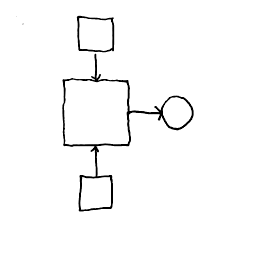
\includegraphics[width = 5cm]{../TikZ/drawings/expert-45.png}&
    
        \begin{minipage}{10cm}
        \begin{verbatim}
  circle(7,6)
    for (2)
            reflect(y = 12)
            line(2*i + 2,4*i + 2,4*i + 2,2*i + 4,arrow = True,solid = True)
            rectangle(-1*i + 1,-6*i + 10,3,-4*i + 12)
        \end{verbatim}
\end{minipage}

    \end{tabular}        
            \\

            \begin{tabular}{ll}
    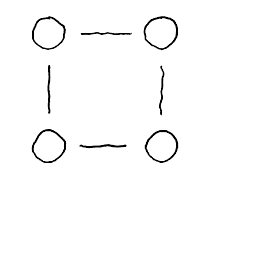
\includegraphics[width = 5cm]{../TikZ/drawings/expert-46.png}&
    
        \begin{minipage}{10cm}
        \begin{verbatim}
      reflect(x = 9)
      line(8,3,8,6,arrow = False,solid = True)
            reflect(y = 9)
            circle(1,1)
            line(3,1,6,1,arrow = False,solid = True)
        \end{verbatim}
\end{minipage}

    \end{tabular}        
            \\

            \begin{tabular}{ll}
    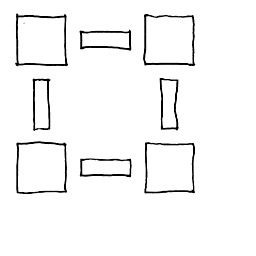
\includegraphics[width = 5cm]{../TikZ/drawings/expert-47.png}&
    
        \begin{minipage}{10cm}
        \begin{verbatim}
      reflect(y = 11)
      rectangle(4,9,7,10)
            reflect(x = 11)
            rectangle(8,0,11,3)
            rectangle(9,4,10,7)
        \end{verbatim}
\end{minipage}

    \end{tabular}        
            \\

            \begin{tabular}{ll}
    
\includegraphics[width = 5cm]{../TikZ/drawings/expert-48.png}&
    
        \begin{minipage}{10cm}
        \begin{verbatim}
  for (3)
      line(3,-1*i + 2,5,-1*i + 2,arrow = False,solid = True)
      line(-1*i + 2,3,-1*i + 4,3,arrow = False,solid = True)
        \end{verbatim}
\end{minipage}

    \end{tabular}        
            \\

            \begin{tabular}{ll}
    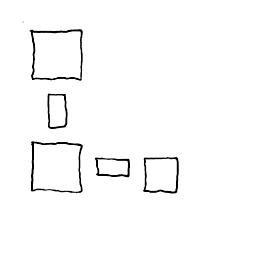
\includegraphics[width = 5cm]{../TikZ/drawings/expert-49.png}&
    
        \begin{minipage}{10cm}
        \begin{verbatim}
  rectangle(0,0,3,3)
    for (2)
        rectangle(0,-3*i + 7,-1*i + 3,-4*i + 10)
        rectangle(-3*i + 7,0,-3*i + 9,2)
        \end{verbatim}
\end{minipage}

    \end{tabular}        
            \\

            \begin{tabular}{ll}
    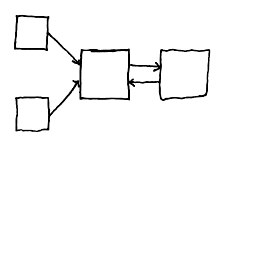
\includegraphics[width = 5cm]{../TikZ/drawings/expert-50.png}&
    
        \begin{minipage}{10cm}
        \begin{verbatim}
  line(8,3,9,3,arrow = False,solid = True)
    for (2)
        line(2,-5*i + 6,4,-1*i + 4,arrow = True,solid = True)
        line(7,-1*i + 4,-2*i + 9,-1*i + 4,arrow = True,solid = True)
        rectangle(0,-5*i + 5,2,-5*i + 7)
        rectangle(-5*i + 9,2,-5*i + 12,5)
        \end{verbatim}
\end{minipage}

    \end{tabular}        
            \\

            \begin{tabular}{ll}
    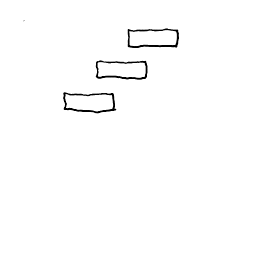
\includegraphics[width = 5cm]{../TikZ/drawings/expert-51.png}&
    
        \begin{minipage}{10cm}
        \begin{verbatim}
  rectangle(4,4,7,5)
  rectangle(0,0,3,1)
  rectangle(2,2,5,3)
        \end{verbatim}
\end{minipage}

    \end{tabular}        
            \\

            \begin{tabular}{ll}
    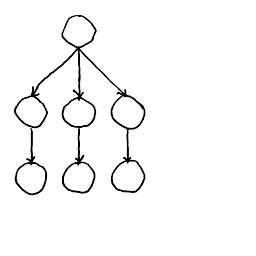
\includegraphics[width = 5cm]{../TikZ/drawings/expert-52.png}&
    
        \begin{minipage}{10cm}
        \begin{verbatim}
  circle(4,10)
    for (3)
        circle(-3*i + 7,5)
        circle(3*i + 1,1)
        line(3*i + 1,4,3*i + 1,2,arrow = True,solid = True)
        line(4,9,-3*i + 7,6,arrow = True,solid = True)
        \end{verbatim}
\end{minipage}

    \end{tabular}        
            \\

            \begin{tabular}{ll}
    \includegraphics[width = 5cm]{../TikZ/drawings/expert-53.png}&
    
        \begin{minipage}{10cm}
        \begin{verbatim}
  line(0,8,8,8,arrow = False,solid = True)
  line(6,8,6,4,arrow = True,solid = True)
  line(2,8,2,6,arrow = True,solid = True)
  line(4,8,4,0,arrow = True,solid = True)
        \end{verbatim}
\end{minipage}

    \end{tabular}        
            \\

            \begin{tabular}{ll}
    \includegraphics[width = 5cm]{../TikZ/drawings/expert-54.png}&
    
        \begin{minipage}{10cm}
        \begin{verbatim}
  line(2,3,2,5,arrow = False,solid = True)
  rectangle(1,5,3,7)
  rectangle(0,0,4,7)
  rectangle(1,1,3,3)
        \end{verbatim}
\end{minipage}

    \end{tabular}        
            \\

            \begin{tabular}{ll}
    \includegraphics[width = 5cm]{../TikZ/drawings/expert-55.png}&
    
        \begin{minipage}{10cm}
        \begin{verbatim}
  circle(1,5)
  line(1,4,1,2,arrow = True,solid = True)
  rectangle(0,0,2,2)
        \end{verbatim}
\end{minipage}

    \end{tabular}        
            \\

            \begin{tabular}{ll}
    \includegraphics[width = 5cm]{../TikZ/drawings/expert-56.png}&
    
        \begin{minipage}{10cm}
        \begin{verbatim}
  circle(3,1)
    for (2)
            reflect(x = 6)
            circle(4*i + 1,-4*i + 8)
            circle(-4*i + 5,5*i + 1)
            rectangle(-4*i + 4,-3*i + 3,6,-7*i + 9)
        \end{verbatim}
\end{minipage}

    \end{tabular}        
            \\

            \begin{tabular}{ll}
    \includegraphics[width = 5cm]{../TikZ/drawings/expert-57.png}&
    
        \begin{minipage}{10cm}
        \begin{verbatim}
  for (3)
      circle(-4*i + 9,4)
      circle(4*i + 1,7)
      circle(-4*i + 9,1)
        \end{verbatim}
\end{minipage}

    \end{tabular}        
            \\

            \begin{tabular}{ll}
    \includegraphics[width = 5cm]{../TikZ/drawings/expert-58.png}&
    
        \begin{minipage}{10cm}
        \begin{verbatim}
  line(8,0,8,7,arrow = True,solid = True)
  line(8,0,0,0,arrow = True,solid = True)
    for (3)
        rectangle(-2*i + 6,0,-2*i + 7,-1*i + 5)
        \end{verbatim}
\end{minipage}

    \end{tabular}        
            \\

            \begin{tabular}{ll}
    \includegraphics[width = 5cm]{../TikZ/drawings/expert-59.png}&
    
        \begin{minipage}{10cm}
        \begin{verbatim}
  line(4,0,0,0,arrow = False,solid = False)
        \end{verbatim}
\end{minipage}

    \end{tabular}        
            \\

            \begin{tabular}{ll}
    \includegraphics[width = 5cm]{../TikZ/drawings/expert-60.png}&
    
        \begin{minipage}{10cm}
        \begin{verbatim}
  rectangle(0,3,2,5)
    for (2)
        circle(3*i + 4,1)
        circle(-2*i + 7,-3*i + 7)
        line(-1*i + 6,-4*i + 7,2*i + 5,-3*i + 5,arrow = True,solid = True)
        line(3*i + 2,-1*i + 4,4,-2*i + 4,arrow = True,solid = True)
        \end{verbatim}
\end{minipage}

    \end{tabular}        
            \\

            \begin{tabular}{ll}
    \includegraphics[width = 5cm]{../TikZ/drawings/expert-61.png}&
    
        \begin{minipage}{10cm}
        \begin{verbatim}
  circle(2,1)
  circle(6,1)
  line(5,1,3,1,arrow = True,solid = True)
  rectangle(0,0,7,2)
        \end{verbatim}
\end{minipage}

    \end{tabular}        
            \\

            \begin{tabular}{ll}
    \includegraphics[width = 5cm]{../TikZ/drawings/expert-62.png}&
    
        \begin{minipage}{10cm}
        \begin{verbatim}
  rectangle(2,1,4,3)
  rectangle(5,0,8,3)
  rectangle(0,2,1,3)
        \end{verbatim}
\end{minipage}

    \end{tabular}        
            \\

            \begin{tabular}{ll}
    \includegraphics[width = 5cm]{../TikZ/drawings/expert-63.png}&
    
        \begin{minipage}{10cm}
        \begin{verbatim}
  rectangle(2,2,3,3)
  rectangle(0,0,5,5)
  rectangle(1,1,4,4)
        \end{verbatim}
\end{minipage}

    \end{tabular}        
            \\

            \begin{tabular}{ll}
    \includegraphics[width = 5cm]{../TikZ/drawings/expert-64.png}&
    
        \begin{minipage}{10cm}
        \begin{verbatim}
      reflect(x = 6)
      line(5,2,5,4,arrow = False,solid = True)
            reflect(y = 6)
            line(2,1,4,1,arrow = False,solid = True)
            rectangle(0,0,2,2)
        \end{verbatim}
\end{minipage}

    \end{tabular}        
            \\

            \begin{tabular}{ll}
    \includegraphics[width = 5cm]{../TikZ/drawings/expert-65.png}&
    
        \begin{minipage}{10cm}
        \begin{verbatim}
      reflect(x = 6)
      line(5,2,5,4,arrow = False,solid = True)
            reflect(y = 6)
            circle(1,1)
            line(2,1,4,1,arrow = False,solid = True)
        \end{verbatim}
\end{minipage}

    \end{tabular}        
            \\

            \begin{tabular}{ll}
    \includegraphics[width = 5cm]{../TikZ/drawings/expert-66.png}&
    
        \begin{minipage}{10cm}
        \begin{verbatim}
  line(0,2,7,2,arrow = False,solid = True)
  line(1,1,6,1,arrow = False,solid = True)
  line(2,0,5,0,arrow = False,solid = True)
        \end{verbatim}
\end{minipage}

    \end{tabular}        
            \\

            \begin{tabular}{ll}
    \includegraphics[width = 5cm]{../TikZ/drawings/expert-67.png}&
    
        \begin{minipage}{10cm}
        \begin{verbatim}
  line(1,5,5,1,arrow = False,solid = True)
  line(1,4,5,0,arrow = False,solid = True)
  rectangle(0,4,1,5)
  rectangle(5,0,6,1)
        \end{verbatim}
\end{minipage}

    \end{tabular}        
            \\

            \begin{tabular}{ll}
    \includegraphics[width = 5cm]{../TikZ/drawings/expert-68.png}&
    
        \begin{minipage}{10cm}
        \begin{verbatim}
  for (3)
      circle(4*i + 1,1)
      rectangle(-4*i + 8,0,-4*i + 10,2)
        \end{verbatim}
\end{minipage}

    \end{tabular}        
            \\

            \begin{tabular}{ll}
    \includegraphics[width = 5cm]{../TikZ/drawings/expert-69.png}&
    
        \begin{minipage}{10cm}
        \begin{verbatim}
      reflect(x = 5)
      circle(1,1)
      line(4,4,4,2,arrow = True,solid = True)
      rectangle(0,4,5,6)
        \end{verbatim}
\end{minipage}

    \end{tabular}        
            \\

            \begin{tabular}{ll}
    \includegraphics[width = 5cm]{../TikZ/drawings/expert-70.png}&
    
        \begin{minipage}{10cm}
        \begin{verbatim}
  circle(3,1)
    for (2)
        line(-4*i + 5,8,-4*i + 5,6,arrow = True,solid = True)
              reflect(x = 6)
              circle(4*i + 1,-4*i + 9)
              line(5,-4*i + 8,2,-3*i + 5,arrow = True,solid = True)
        \end{verbatim}
\end{minipage}

    \end{tabular}        
            \\

            \begin{tabular}{ll}
    \includegraphics[width = 5cm]{../TikZ/drawings/expert-72.png}&
    
        \begin{minipage}{10cm}
        \begin{verbatim}
      reflect(x = 8)
      circle(4,4)
            reflect(y = 8)
            circle(7,7)
            rectangle(2,2,3,3)
        \end{verbatim}
\end{minipage}

    \end{tabular}        
            \\

            \begin{tabular}{ll}
    \includegraphics[width = 5cm]{../TikZ/drawings/expert-74.png}&
    
        \begin{minipage}{10cm}
        \begin{verbatim}
  rectangle(0,0,6,6)
        reflect(x = 6)
        rectangle(2,2,4,4)
          for (3)
              circle(3,2*i + 1)
              circle(5,-2*i + 5)
        \end{verbatim}
\end{minipage}

    \end{tabular}        
            \\

            \begin{tabular}{ll}
    \includegraphics[width = 5cm]{../TikZ/drawings/expert-75.png}&
    
        \begin{minipage}{10cm}
        \begin{verbatim}
  for (3)
      line(4*i + 2,5,4*i + 4,5,arrow = True,solid = True)
            reflect(x = 10)
            circle(-4*i + 13,1)
            circle(4*i + 5,5)
            line(4*i + 5,4,4*i + 5,2,arrow = True,solid = True)
        \end{verbatim}
\end{minipage}

    \end{tabular}        
            \\

            \begin{tabular}{ll}
    \includegraphics[width = 5cm]{../TikZ/drawings/expert-76.png}&
    
        \begin{minipage}{10cm}
        \begin{verbatim}
  line(4,5,4,10,arrow = False,solid = True)
        reflect(x = 8)
        circle(4,1)
        circle(1,8)
        line(4,5,8,2,arrow = False,solid = True)
        \end{verbatim}
\end{minipage}

    \end{tabular}        
            \\

            \begin{tabular}{ll}
    \includegraphics[width = 5cm]{../TikZ/drawings/expert-77.png}&
    
        \begin{minipage}{10cm}
        \begin{verbatim}
      reflect(x = 10)
      line(6,8,8,8,arrow = False,solid = True)
        for (2)
            circle(-4*i + 5,7*i + 1)
            line(3*i + 6,4*i + 1,9,4*i + 3,arrow = False,solid = True)
            rectangle(4*i + 4,-4*i + 7,4*i + 6,-4*i + 9)
        \end{verbatim}
\end{minipage}

    \end{tabular}        
            \\

            \begin{tabular}{ll}
    \includegraphics[width = 5cm]{../TikZ/drawings/expert-78.png}&
    
        \begin{minipage}{10cm}
        \begin{verbatim}
  line(0,6,12,6,arrow = False,solid = True)
  line(6,6,6,5,arrow = True,solid = True)
  line(8,3,7,4,arrow = True,solid = True)
  line(3,2,5,4,arrow = True,solid = True)
        line(0,8,8,0,arrow = False,solid = True)
        \end{verbatim}
\end{minipage}

    \end{tabular}        
            \\

            \begin{tabular}{ll}
    \includegraphics[width = 5cm]{../TikZ/drawings/expert-81.png}&
    
        \begin{minipage}{10cm}
        \begin{verbatim}
  rectangle(9,0,11,2)
  rectangle(6,0,8,2)
        reflect(x = 5)
        circle(4,1)
        \end{verbatim}
\end{minipage}

    \end{tabular}        
            \\

            \begin{tabular}{ll}
    \includegraphics[width = 5cm]{../TikZ/drawings/expert-83.png}&
    
        \begin{minipage}{10cm}
        \begin{verbatim}
  for (2)
      line(-4*i + 7,6,-6*i + 8,5,arrow = True,solid = True)
            reflect(x = 10)
            circle(2*i + 7,7)
            circle(3*i + 2,-3*i + 4)
            line(7*i + 1,-3*i + 6,3*i + 2,-3*i + 5,arrow = True,solid = True)
        \end{verbatim}
\end{minipage}

    \end{tabular}        
            \\

            \begin{tabular}{ll}
    \includegraphics[width = 5cm]{../TikZ/drawings/expert-85.png}&
    
        \begin{minipage}{10cm}
        \begin{verbatim}
  circle(1,1)
    for (3)
        circle(1,-3*i + 10)
        line(1,-3*i + 9,1,-3*i + 8,arrow = True,solid = True)
        \end{verbatim}
\end{minipage}

    \end{tabular}        
            \\

            \begin{tabular}{ll}
    \includegraphics[width = 5cm]{../TikZ/drawings/expert-86.png}&
    
        \begin{minipage}{10cm}
        \begin{verbatim}
  for (2)
      rectangle(-7*i + 7,-7*i + 7,-7*i + 8,-7*i + 8)
      rectangle(-6*i + 6,-2*i + 4,-6*i + 8,-2*i + 6)
      rectangle(-5*i + 5,5*i,-5*i + 8,5*i + 3)
        \end{verbatim}
\end{minipage}

    \end{tabular}        
            \\

            \begin{tabular}{ll}
    \includegraphics[width = 5cm]{../TikZ/drawings/expert-87.png}&
    
        \begin{minipage}{10cm}
        \begin{verbatim}
      reflect(x = 8)
      rectangle(0,0,1,1)
      rectangle(0,2,2,4)
      rectangle(0,5,3,8)
        \end{verbatim}
\end{minipage}

    \end{tabular}        
            